\chapter{Introduzione alla logica e al linguaggio matematico}
Per capire cosa stiamo trattando proviamo subito a risolvere il seguente problema.
\begin{figure}[ht]
    \centering
    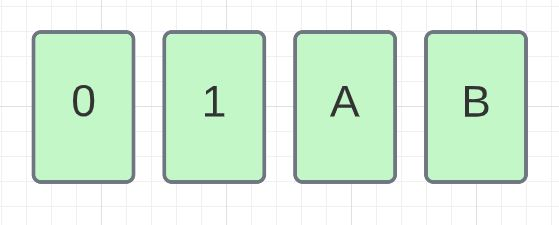
\includegraphics[width = 8cm]{images/carte.JPG}
    \caption{Carte del problema}
    \label{carte}
\end{figure}

\fbox{\parbox[c]{0.9\textwidth}{
    \textit{\\Preso un mazzo, formato da carte aventi una faccia con una lettera dell'alfabeto e l'altra con un numero, dobbiamo verificare quando viene soddisfata la seguente condizione: \textbf{"Se su una faccia della carta si trova una vocale, allora sulla faccia opposta c'è un numero pari".}}\\
}}\\\\Cosiderando le carte in figura \ref{carte}, quali carte devo girare per verificare la veridicità della frase?

Dopo aver risposto a questo primo problema, passiamo al secondo.

\fbox{\parbox[c]{0.9\textwidth}{
    \textit{\\In un bar vige la seguente regola: \textbf{"Può bere alcolici solo chi ha più di 18 anni".} Nel bar ci sono quattro persone, un uomo esplicitamente anziano, un ragazzino con meno di 18 anni, una persona che beve un gin e una persona che beve una Coca-Cola.}\\
}}\\\\Cosiderando quanto descitto, quali persone devo far girare per verificare la condizione imposta dal bar?

La maggior parte delle persone danno risposte diverse ai due problemi. Ma vi stupirà sapere che in realtà i due quesiti sono identici. Le risposte ad entrambi i problemi sono infatti \textbf{NO, SI, SI, NO}.

Benvenuti nel fantastico mondo della logica!!!